\section{Modeling}\label{sec:modeling}
In order to address the two main issues with using OPAL opacity tables we use
our OPLIB opacity table web scraper to generate a set of tables that
consistently model lower metallicities. Specifically, we generate tables for
$Z_{\odot}=0.017$, $Z=0.01$, $Z=0.001$, and $Z=0.0001$. Compositions are
derived from the GS98 solar composition, with the mass fractions between metals
remaining constant, and only the total metal mass fraction is allowed to vary.
Moreover, Helium mass fraction is held constant as extra mass from the reduced
metallicity is put into additional Hydrogen. 

For each metallicity 101, uniformly spaced, models from 0.3 to 0.5 M$_{\odot}$
(spacing of 0.001 M$_{\odot}$) are evolve with both the GS98 OPAL opacity table
and OPLIB tables, hereafter these are the ``coarse'' models. For each set of
coarse models the discontinuity in the mass-luminosity relation is identified
at an age of 7 Gyr (Figures \ref{fig:coarseMassLum} \& \ref{fig:coarseTeffLum}
shows a characteristic example).

Immediately, the difference in mass where the discontinuity manifests is clear.
For each metallicity the discontinuity in the OPLIB models is approximately one
one-hundredth of a solar mass lower than the discontinuity in the OPAL models. We can
validate that this discontinuity is indeed correlated with the convective
transition mass; Figure \ref{fig:convTransition} shows an example of the model
forming radiative zones at approximately the same masses where the discontinuity
in the mass-luminosity function exists.

At this resolution only a few models exist within the
mass range of the discontinuity. In order to better constrain its location we
run a series of ``fine'' models, with a mass step of 0.0001 M$_{\odot}$ and
ranging from where the mass derivative first exceeds two sigma away from the
mean derivative value up to the mass where it last exceeds two sigma away from
the mean. A characteristic fine mass-luminosity relation is shown in Figure
\ref{fig:fineMassLum}.


\begin{figure}
	\centering
	\vspace{5mm}
	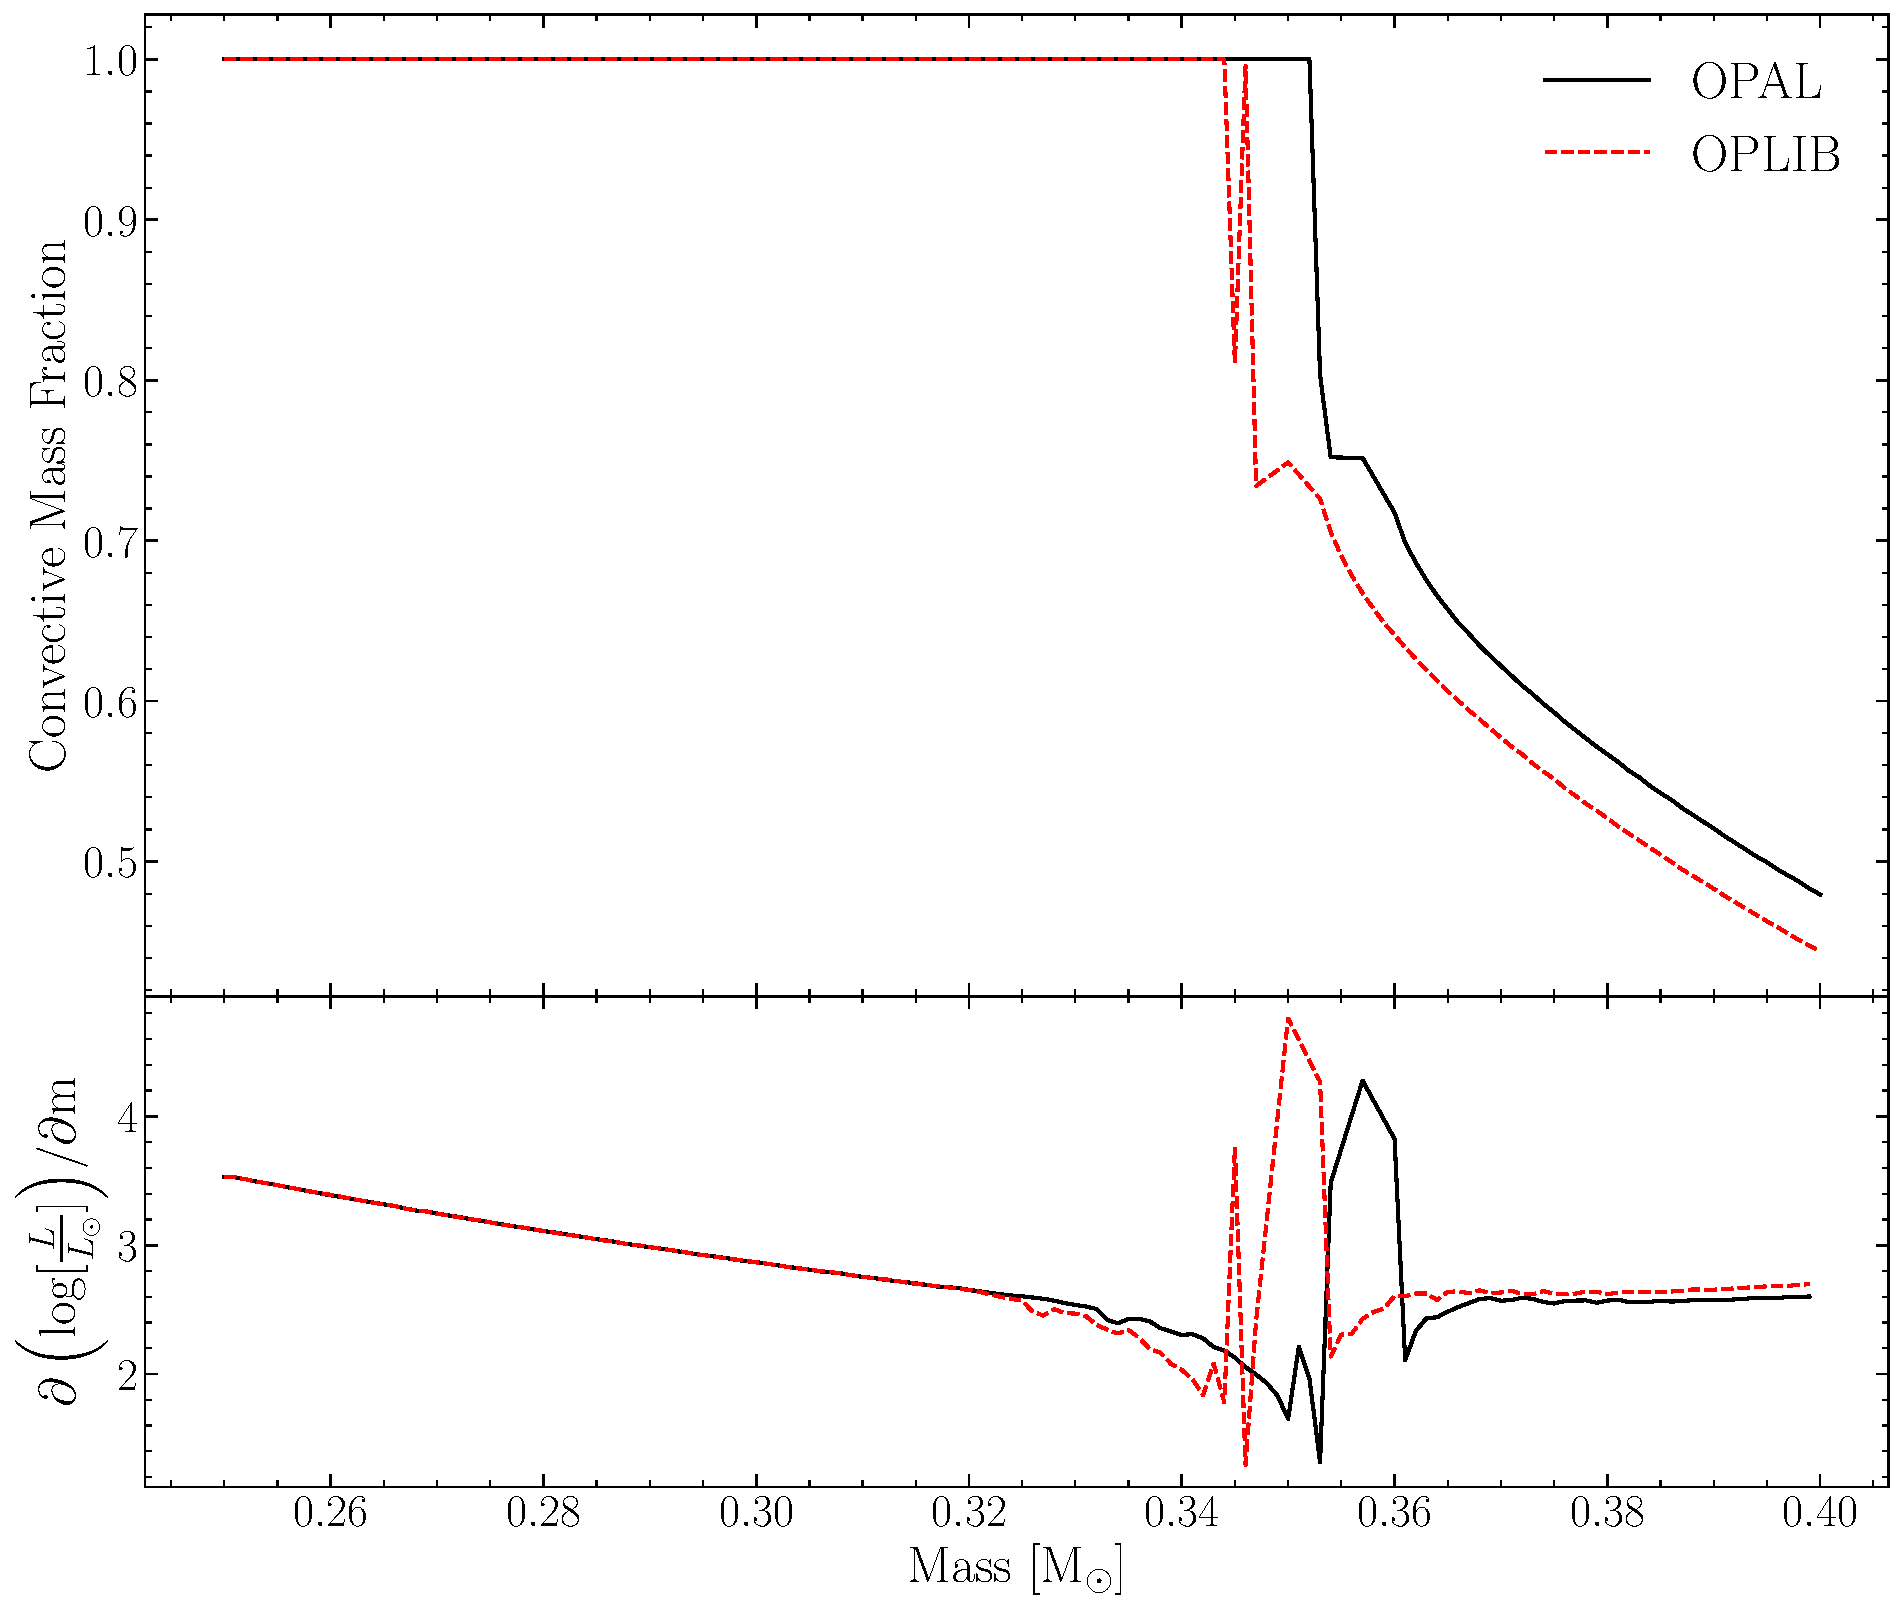
\includegraphics[width=0.45\textwidth]{src/figures/ConvectiveMassFraction.pdf}
	\caption{Convective Mass Fraction vs. initial model mass for Z=0.01 at 7
	Gyr (top), Derivative of luminosity with respect to mass for the OPAL and
	OPLIB models (bottom).  Note how the model transitions from fully
	convective at approximately the same mass where the discontinuity exists.}
	\label{fig:convTransition}
\end{figure}


\begin{figure}
	\centering
	\vspace{5mm}
	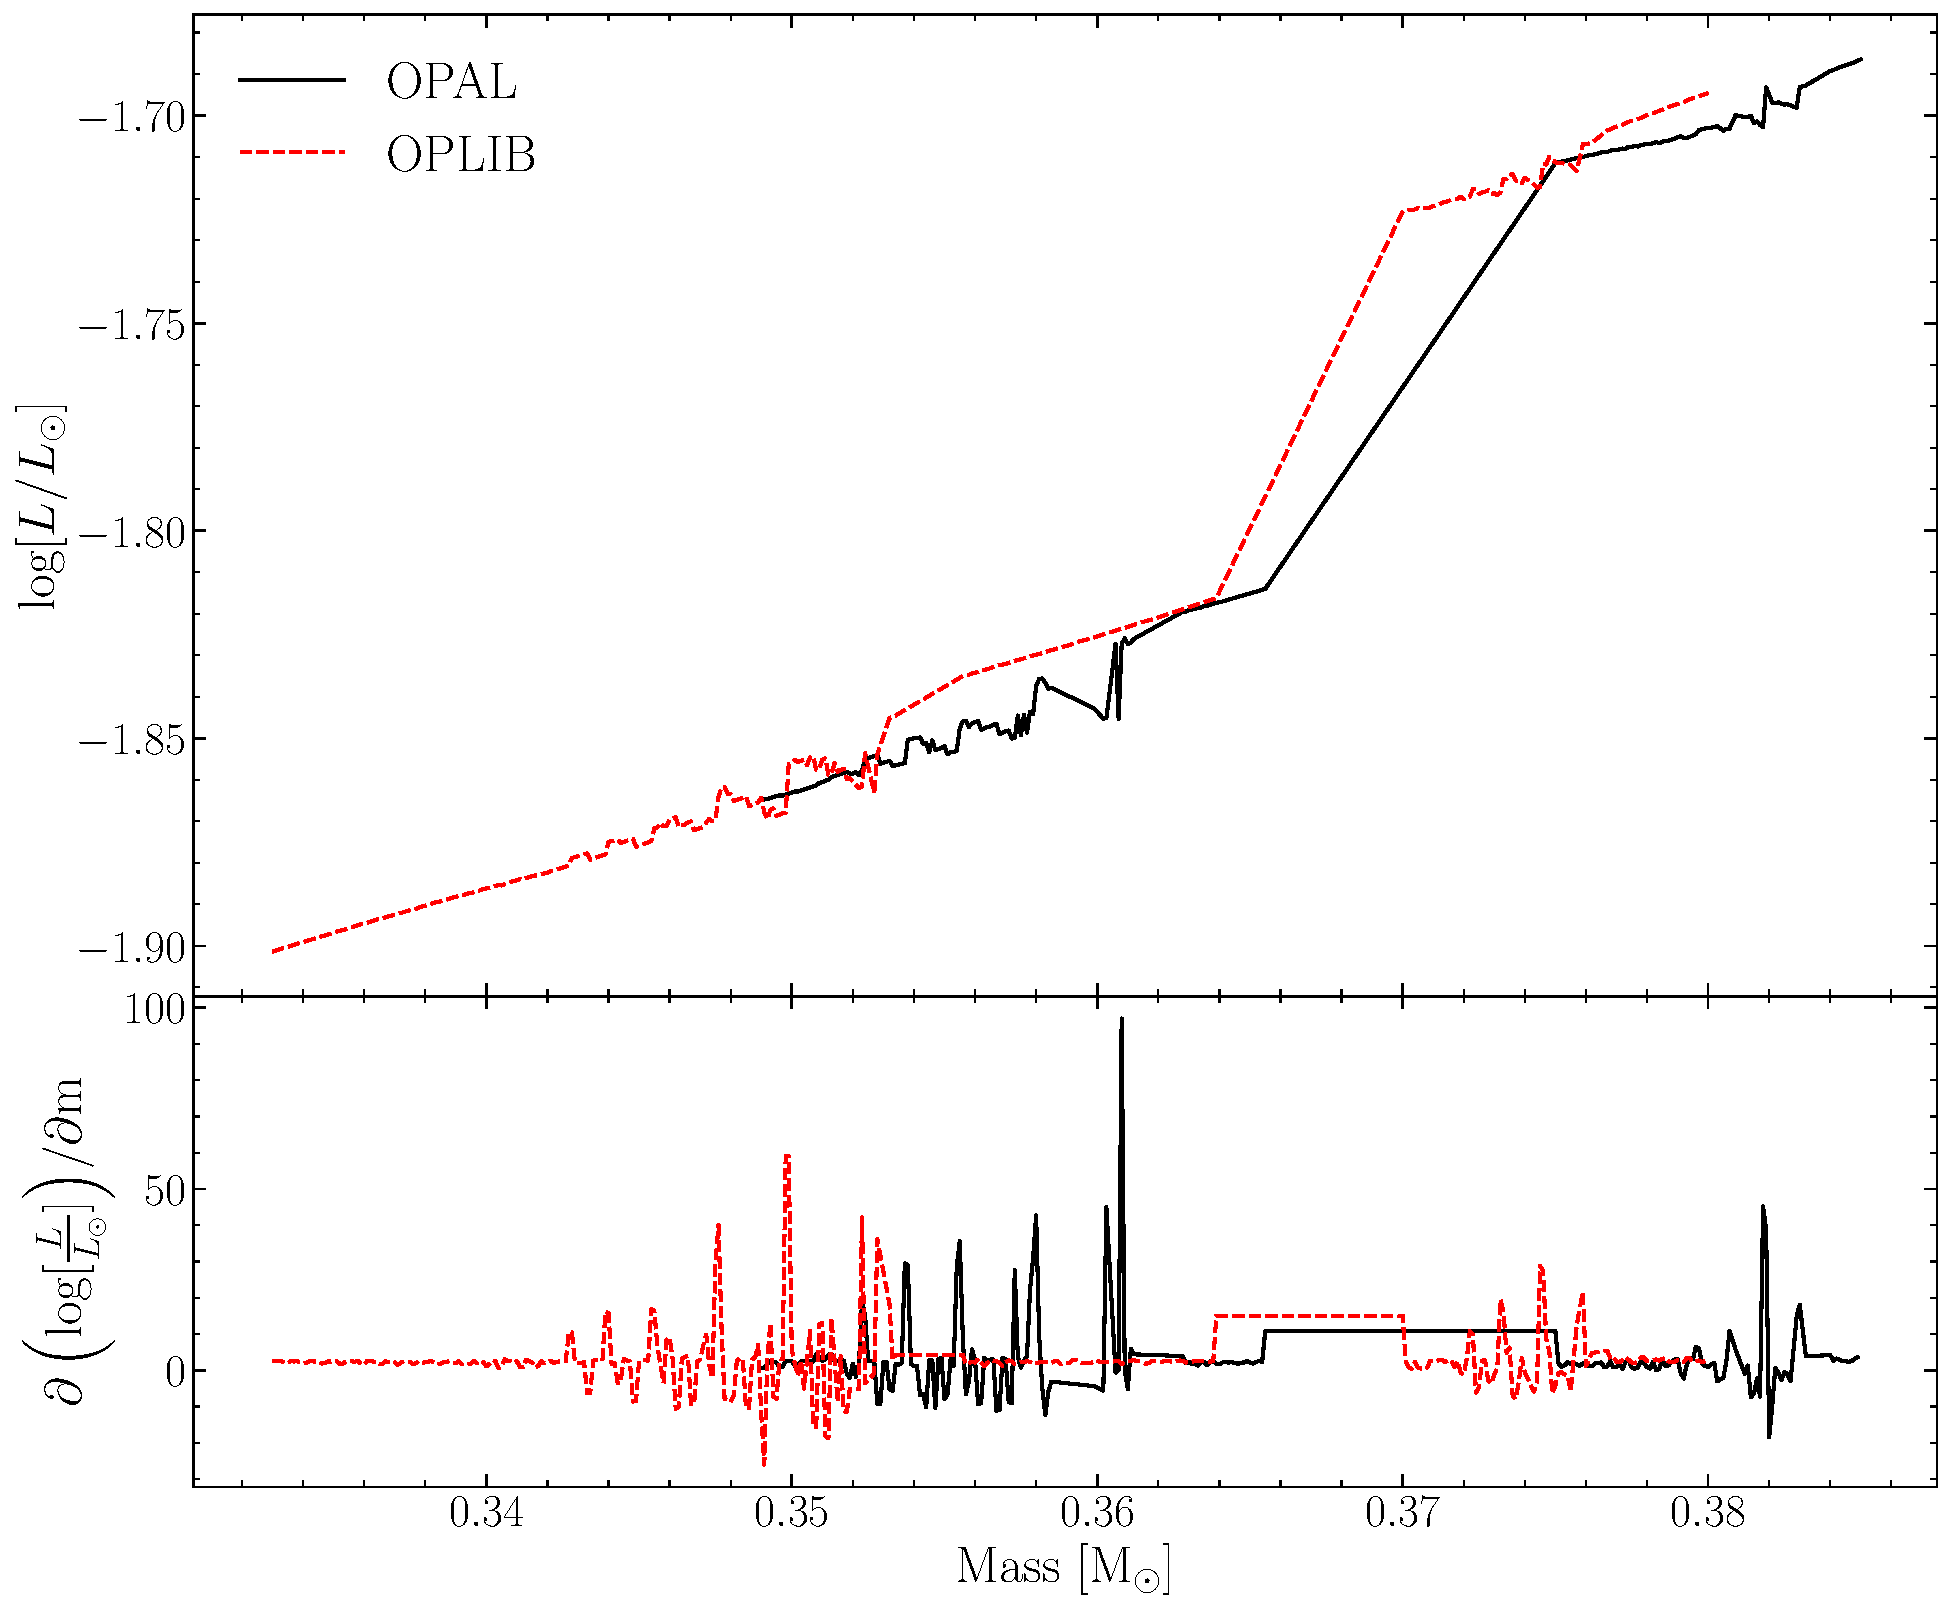
\includegraphics[width=0.45\textwidth]{src/figures/MassLumDisconZ001Paper-fine.pdf}
	\caption{Mass-Luminosity relation for Z=0.01 at 7 Gyr for models run with
	both OPAL and OPLIB high-temperature opacity tables and a mass step between
	them of 0.0001 M$_{\odot}$ (top). Derivative of luminosity with respect to
	mass for the OPAL and OPLIB models (bottom).}
	\label{fig:fineMassLum}
\end{figure}

Using the fine models we identify the location of the discontinuity in the same
manner as before, results of this are presented in Table
\ref{tab:fineMassRange}. Of note with the mass ranges we measure for the
discontinuity is that are generally not in agreement with those measured in
\citet{Mansfield2021}. However, the luminosity difference from over the gap
($\approx 0.1 mag$) is similar to both the observational difference and that
reported in \citet{Mansfield2021}. Currently, it is not clear why our mass
range is not in agreement with the \citet{Mansfield2021} mass range and further
investigation is therefore needed.
